\section{System Architecture}
The system architecture defines the structure and behaviour of a system. IAFoosball is a solution for an interactive user experience for foosball. It thus compromises a cloud part, an edge part and a constrained device (IoT part). This is shown in \cref{fig:systemArch}. We will focus on the edge and IoT part and only brievly touch on the cloud part for completness. 
\begin{figure}[h!]
    \centering
    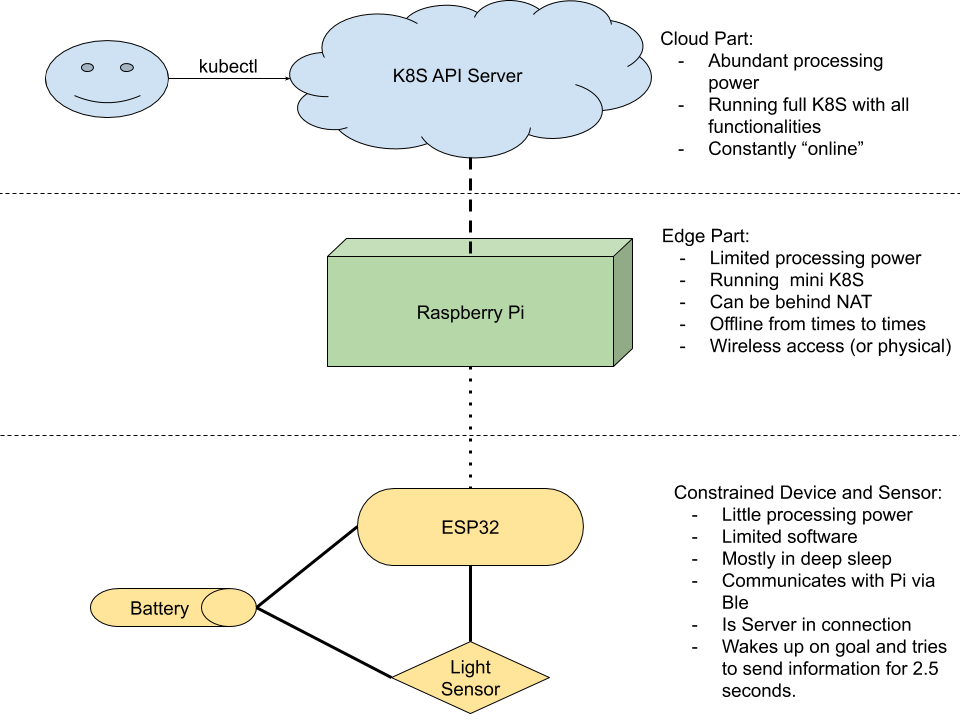
\includegraphics[scale=0.3]{figures/system-arch.png}% picture filename
    \caption{The System Architecture}\label{fig:systemArch}
\end{figure}\\
The cloud is where all user relevant data is stored and where the system is administered. It runs on Kubernetes, which abstracts the physical hardware programs run on and puts them into pods. Pods are smalles unit in Kubernetes and are isolated into their own namespace and cgroup and can contain multiple containers. Unlike virtual machine, it does not create any overhead at runtime for containers, but t offers the possibility to fully orchestrate the pods. This means, pods can restarted if they are not behaving correctly, replicas can be turned up or down depending on the system load, it offers automated rollouts and the Kubernetes itself is highly extensable.\\
Kubernetes was developed as a cloud platform, but as edge devices become more powerful and do more processing of data, especially executing business logic, managin them is becoming an increasingly popular research topic. Processing at the edge is called edge (or fog) computing and has many challenges. The edge devices can have very limitted power, they can be offline from time to time, have a slow Internet connection and be behind a NAT. Kubernetes was not designed to be used on the edge, but because its extension model, engineers are now working exactly on that. This means, an edge device can be just another node inside network, treated differently than other nodes though, but still containing all the advantages Kubernetes offers.\\
Last but most importantly, the IoT part is where the actual sensing of the data happens. This device is so processing power restricted that it can not run Kubernetes, but updates for it can be build inside a container running either in the cloud or on the raspberry and pushed to the microcontroller via a OTM update. This makes updating multiple devices feasable and ensures that updates, especially security updates, can be rolled out quickly.\\
The actual architecture of the goal is compromised of the esp32, a battery and the laser and a photon resistor. When a goal is scored, meaning the laser does not shine on the resistor, a goal is registered. The esp32 then opens a ble server and notifies the edge device of the goal. How this is exactly done is discussed after the testing chapter. If the rpi acknowledges the goal, the 
Laser always on???

